%% LyX 2.0.7.1 created this file.  For more info, see http://www.lyx.org/.
%% Do not edit unless you really know what you are doing.
\documentclass[english]{llncs}
\usepackage[T1]{fontenc}
\usepackage[latin9]{inputenc}
\usepackage{array}
\usepackage{verbatim}
\usepackage{url}
\usepackage{multirow}
\usepackage{graphicx}
\PassOptionsToPackage{normalem}{ulem}
\usepackage{ulem}
\usepackage{epstopdf} 
\usepackage{color} 

\makeatletter

%%%%%%%%%%%%%%%%%%%%%%%%%%%%%% LyX specific LaTeX commands.
%% Because html converters don't know tabularnewline
\providecommand{\tabularnewline}{\\}

%%%%%%%%%%%%%%%%%%%%%%%%%%%%%% User specified LaTeX commands.
\usepackage{algorithmic}

\@ifundefined{showcaptionsetup}{}{%
 \PassOptionsToPackage{caption=false}{subfig}}
\usepackage{subfig}
\makeatother

\usepackage{babel}
\begin{document}
\title{{A Study of Query Reformulation for Patent Prior Art Search with Partial Patent Applications}}
\maketitle
\begin{abstract}
Patents are used by entities to legally protect their inventions and
represent a multi-billion dollar industry of licensing and litigation.
In 2012, 276,788 patent applications were approved in the US alone
-- a number that has doubled in the past 15 years. While much of the
literature inspired by the evaluation framework of the CLEF-IP competition
has aimed to assist patent examiners in assessing prior art for complete
patent applications, less of this work has focused on patent search
with queries representing (partial) applications to help inventors
to assess the patentability of their ideas prior to writing a full
application. %Hence, in this paper, we focus on both helping inventors to assess the patentability of their ideas and patents examiners to assess the patentability of a given patent application.
In this paper, we carry out an intensive study of query reformulation
for patent prior art search with partial patent applications, with
the objective of assessing not only the performance of standard query
reformulation methods, but also the effectiveness of query reformulation
methods that exploit patent-specific characteristics. We also propose
new query reformulation methods that (a) exploit patent structure
and (b) leverage techniques for diverse term selection in query reformulation.
We demonstrate that our methods improve both general (MAP) and patent-specific
(PRES) evaluation metrics for prior art search performance on standardized
datasets of CLEF-IP, with respect to both general and specific query
reformulation methods. 
\end{abstract}
\begin{keywords} Query Reformulation, Patent Search. \end{keywords} 





\section{Introduction}

\noindent Patents are used by entities to legally protect their inventions
and represent a multi-billion dollar industry of licensing and litigation.
In 2012, 276,788 patent applications were approved in the US alone
a number that has doubled in the past 15 years. Hence, helping both
inventors and patent examiners assess the patentability of a given
patent application through a patent prior art search is a critical
task.

Patent prior art search involves finding previously granted patents
that may be relevant to a new patent application. The objective and
challenges of standard formulations of patent prior art search are
different from those of standard text and web search since~\cite{Magdy2012}:
(i) queries are (partial) patent applications, which consist of documents
with hundreds of words organized into several sections, while queries
in text and web search constitute only a few words; (ii) patent prior
art search is a recall-oriented task, where the primary focus is to
retrieve all relevant documents at early ranks, in contrast to text
and web search that are precision-oriented, where the primary goal
is to retrieve a subset of relevant documents.
Another important characteristic about patent patent prior art search
is that, in contrast to scientific and technical writers, patent
writers tend to generalize and maximize the scope of what is protected
by a patent,
%by using a combination of abstract and specific terminology, 
and try to make sure that finding any relevant prior
work by the patent examiner is a hard job.

While much of the literature inspired by the evaluation framework
of the CLEF-IP competition has aimed to assist patent examiners in
assessing prior art for complete patent applications, less work has
focused on assessing the patentability of inventions before writing
a full patent application. Prior art search with queries that represent
unfinished patent applications is certainly desirable, since writing
a full application is time-consuming and costly, especially if lawyers
are hired to assist.

%However prior art search with partial applications is much different than queries with a full application -- namely because the queries are much shorter and represent only parts of a patent application.


%NOTE: start a paragaph with the key idea
%A patent application is organized in, at least, four sections: title,
%abstract, claims and description. We assumed that a partial application
%consist in one of the mentioned sections. 
To assess the difficulty of querying with partial patent applications,
we refer to Figure~\ref{fig:FailureAnalysis}. Here we show an analysis
of the average Jaccard similarity%
\footnote{The Jaccard similarity is used to measure the term overlap between
two sets, and is defined as the size of the intersection divided by
the size of the union of the sample sets. Before applying the Jaccard
similarity, patent-specific stopwords were removed, as suggested by
\cite{Mahdabi2012}.%
} between different queries (representing the title, abstract, claims,
or descriptions intended to represent a partial patent application)
and the labeled relevant (all) and irrelevant documents (top 10 irrelevant
documents ranked by BM25~\cite{Robertson1993}). We show results
for the top 100 and bottom 100 queries (100 queries that perform the
best, and 100 queries that perform the worst) of CLEP-IP 2010 evaluated
according to Mean Average Precision (MAP).
Note that, while the title section is usually composed by an average of six terms, the
other sections are longer, ranging from ten to thousands of terms.


\begin{figure}[!th]
\begin{centering}
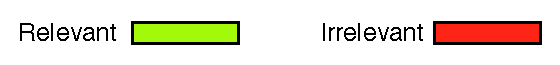
\includegraphics[width=4.5cm]{img/legend} 
\par\end{centering}

\begin{centering}
\subfloat[Title query.]{\begin{centering}
\includegraphics[width=3cm]{Results-CIKM2014/jaccard-qTitle-CLEF-IP2010}
\par\end{centering}

}\subfloat[Abstract query.]{\begin{centering}
\includegraphics[width=3cm]{Results-CIKM2014/jaccard-qAbstract-CLEF-IP2010}
\par\end{centering}

}\subfloat[Claims query.]{\begin{centering}
\includegraphics[width=3cm]{Results-CIKM2014/jaccard-qClaims-CLEF-IP2010}
\par\end{centering}

}\subfloat[Description query.]{\begin{centering}
\includegraphics[width=3cm]{Results-CIKM2014/jaccard-qDescription-CLEF-IP2010}
\par\end{centering}

} \caption{Average Jaccard similarity of (ir)relevant documents with the result
sets for different queries. }

\par\end{centering}

{\footnotesize{}{}%different queries (representing the title, abstract, or claims of a patent application)
%and the labeled (ir)relevant documents for the best (top) and worst (bottom) performing
%queries from CLEF-IP 2010 w.r.t. MAP.}
\label{fig:FailureAnalysis}} 
\end{figure}


There are three notable trends here: (i) term overlap increases from title to description since the query size grows accordingly; (ii) the bottom 100 performing queries tend to have much smaller term overlap with the relevant documents than the top 100 queries; and (iii) the best overlap for any relevant document set for any set of queries is less than one in four terms.
Therefore, we suggest an investigation of \emph{query
reformulation} \cite{Baeza-Yates2010} methods as a means for improving
the term overlap between queries that represent partial patent applications and relevant documents, with the
objective of assessing not only the performance of standard query
reformulation methods, but also the effectiveness of query reformulation
methods that exploit patent-specific characteristics. 

The rest of the paper is organized as follows: 
in Section \label{sec:relatedworks} we present the related work,
in Section \ref{sec:QueryReformulationForPatents}
we present query reformulation frameworks; in Section \ref{sec:evaluation}
we present our evaluation framework and results analysis; and in Section
\ref{sec:conclusion} we conclude with possible directions for future
work.

%Query Reformulation is the process of transforming an initial query $Q$ to another query $Q'$. This transformation may be either a reduction or an expansion of the query. \emph{Query Reduction} (QR) \cite{Kumaran2009} reduces the query such that superfluous information is removed, while \emph{Query Expansion} (QE) \cite{Efthimiadis1996} enhance the query with additional terms likely to occur in relevant documents. 

%Therefore, we investigate the impact of query reduction methods when querying with long sections such as abstract, claims or description. 

%As already mentioned, Query Expansion (QE)~\cite{Efthimiadis1996} is a query reformulation approach that adds terms to an initial query in order to improve retrieval performance. The utility of QE for patent prior art search is motivated by the term overlap analysis depicted in Figure \ref{fig:FailureAnalysis}, which illustrates that there is a large term mismatch between queries an relevant documents. This term mismatch may be alleviated by QE methods.

% The following is a reasonable argument, but could be refuted by
% reviewers... term coverage and recall are more direct and simple
% arguments.



%In summary, the contributions of this paper are the following:  
%\begin{enumerate}
%\item Novel contributions for query expansion and reduction that leverage
%(a) patent structure and (b) term diversification techniques. 
%\item A thorough comparative analysis of existing and novel methods for
%query expansion and reduction in patent prior-art search on standardized
%datasets of CLEF-IP. 
%\end{enumerate}



\section{Related work}
\label{sec:relatedworks}

{\color{red} Gaby said: this section should be shorter}

Query Reformulation is the process of transforming an initial query $Q$ to another query $Q'$. This transformation may be either a reduction or an expansion of the query. \emph{Query Reduction} (QR) \cite{Kumaran2009} reduces the query such that superfluous information is removed, while \emph{Query Expansion} (QE) \cite{Efthimiadis1996} enhance the query with additional terms likely to occur in relevant documents. 

%The major contributions in patent search has focused on query formulation, where the objective is to find the best terms to represent a patent application as a query to achieve high retrieval effectiveness by retrieving all possible relevant documents at high ranks \cite{Magdy2012}. 

%The scenario of patent prior art search consists of manually form queries by selecting high frequency terms from patent application. Hence, following this methodology, some algorithms of patent query reduction have been proposed to select only useful terms from patent application \cite{Ganguly2011,Itoh2003}. We used the approach propose by Ganguly et al. \cite{Ganguly2011} for QR as a baseline, and we showed that the performance of MMRQR outperform this approach in many cases. 

\begin{comment}
There are a variety of existing query expansion methods that use synonyms
(both from WordNet and automatically generated)~\cite{Magdy2011},
by supervised learning~\cite{Bashir2010}, by IPC codes (a variant
on our baseline approach that additionally uses the citation network
of patents)~\cite{Verma2011}, and a query-specific patent lexicon
based on the definitions of the IPC~\cite{Mahdabi2013}. While our
intention in this paper was to comprehensively evaluate very general
methods for QE using \emph{partial patent applications}; it would
be interesting future work to comprehensively evaluate all of these
patent-specific QE methods with our generic methods for partial patent
application queries. 
\end{comment}

Classical query expansion methods has been used for prior art search by 
Magdy et al. \cite{Magdy2011}, which rely on pseudo-relevance feedback and WordNet as
source of expansion terms. However, none of these approaches were
able to achieve a significant improvement over the baseline. Therefore,
they introduce a novel approach that automatically generates synonym
sets for terms, and use them as a source of expansion terms, which
showed significant improvement with respect to the baseline. 
Also, Bashir et al. \cite{Bashir2010} propose a query expansion with pseudo-relevance
feedback. Query expansion terms are selected using a using a machine
learning approach, by picking terms that may have a potential positive
impact on the retrieval effectiveness. However, this approach can
be computational expensive, since the presented features are complicated
to compute, e.g. Pair-wise Terms Proximity features. 
Verma and Varma \cite{Verma2011} propose a different approach, which instead of using
the patent text to query, use its International Patent Classification
(IPC) codes, which are expanded using the citation network. The formed
query is used to perform an initial search. The results are then re-ranked
using queries constructed from patent text. Throughout our experiments,
we concluded that relying on non-patent terms to expand a query, leads to poor retrieval quality.
Lastly, a more recent work by Mahdabi et al. \cite{Mahdabi2013} propose to combine query reduction and xpansion method for prior art search.
For query reduction, they shorten the query by taking only the first claim since it contains the core of the invention.
For the query expansion, they built a query-specific patent lexicon based on the definitions of the IPC. Then, the patent lexicon is used to select expansion terms that are focused on the reduced query.
Lastly, a more recent work by Mahdabi et al. \cite{Mahdabi2013} propose
a query expansion method that build a query-specific patent lexicon
based on the definitions of the IPC. Then, this patent lexicon is
used to select expansion terms that are focused on the query topic. 

Also query reduction methods have been applied in order to deal with long queries, 
which are composed by full patent applications \cite{Ganguly2011,Itoh2003}. Even these methods are interesting, they are not suited to deal with short queries (partial patent applications).
\cite{Ganguly2011} technique decomposes a query
(a patent section) into constituent text segments and computes the
Language Modeling (LM) similarities by calculating the probability
of generating each segment from the top ranked documents (PRF set).
Then, the query is reduced by removing the least similar segments
from the query. Recently, \cite{Mahdabi2013} proposed as reduction process to short
the query by taking only the first claim of a patent application since
it contains the core of the invention. This approach has not been
implemented as its authors already point out its poor performance.





\section{Query Reformulation for patents}
\label{sec:reformulation}

%In this section, we first present the requirements of a query expansion method in Sections \ref{sec:FrameworkQE}, then, we introduce a novel term selection method for query expansion in Section \ref{sec:MMRQE}. Next, in Section \ref{sec:FrameworkQR} we introduce the motivations behind the benefit of query reduction, and a new approach of query reduction in Section \ref{sec:MMRQR}.
During the exploration of query reformulation for patent search with
partial patent applications, there are many configuration options
and associated questions that we considered: 


\begin{description}
\item [{Query type:}] We consider that a query of a partial patent application
consist of either the title, the abstract, the claims or the description
section. %\footnote{A query is always evaluated against the full content (title, abstract, claims, description) of granted patent applications since it is sensible to make use of all available content.}
A critical question is what part of a partial application an inventor
should write to obtain the best search results? %(ii) \textbf{what part of a patent application a patent examiner should use to make a patent prior art search? }

\item [{Relevance model:}] %For initial retrieval of documents in the \emph{pseudo-relevant} feedback set (PRF) %---\textbf{ often used to generate the terms for QE} --- and subsequent re-retrieval, there are various options for the relevance ranking model. 
We explore a probabilistic approach represented
by the popular BM25~\cite{Robertson1993} algorithm, as well as a
vector space model (VSM) approach, TF-IDF~\cite{Salton1975}. A natural
question is which relevance model works best for query reformulation
for patent prior art search? 

\item [{Query expansion source:}] We consider the title, abstract, claims,
and description sections as different term sources to determine which
section offers the best source of expansion terms, e.g., are the title
words of particularly high value as expansion terms? 
In addition we included two
other patent specific QE methods as baselines. Motivated by \cite{Mahdabi2013},
we used the text definitions of the International Patent Classification
(IPC) codes assigned to a patent application as a source for query
expansion --- this is denoted as \textbf{IPC Codes}. We also implemented
the two variants of the QE approach proposed in \cite{Magdy2011}, which automatically generates candidate synonyms sets (SynSet) for terms, and use it as
a source of expansion terms, which are denoted as \textbf{WSynSet}) and 
\textbf{USynSet}). Note that this only applies to query expansion methods. 


\item [{Term selection method:}] We consider different term selection
methods for query reformulation. We evaluate the performance of term
selection using Rocchio~\cite{Salton1971} and new term selection
methods that we propose in the next sections. %,which is intended to address the high-recall nature of patent prior art search. 
Then a natural question is, which term selection method works best,
and with which configuration, i.e. query type, retrieval model, and
term source for query expansion methods? 

\item[{Query reduction method:}] As a general QR method, we proposed to adapt the Rocchio method for query pruning. Basically, the idea is once we have computed the Rocchio
modified query vector, we take only terms of the initial query that
appear in this vector and rank them using the Rocchio score. Then,
we remove $n$ terms with the lower score. We refer to this approach
as \textbf{RocchioQR}. 
We also proposed a baseline method that use IPC codes for query reduction
as follows: (i) For each patent application, we take the definitions
of the IPC codes which are associated to it. Then, (ii) we rank the
terms of the query according to both their frequency in the class
code definition, and their frequency in the query. Finally, (iii)
we remove bottom terms of this ranking from the query (i.e. good terms
are terms that occur a lot in the query, and few in the class code
definition, whereas bad terms are those that occur few in the query,
and a lot in the class code definition). The intuition is that, terms
in the IPC code definition may represent \textquotedbl{}stopwords\textquotedbl{},
especially if they are rare (infrequent in the patent application).
We denote this approach \textbf{StopIPC Codes}.
\end{description}


In summary, .....

\begin{itemize}
\item \textbf{\footnotesize{}{}Query type:}{\footnotesize{}{} $\{\mathrm{Title},\mathrm{Abstract},\mathrm{Claims},\mathrm{Description}\}$ }{\footnotesize \par}

\item \textbf{\footnotesize{}{}Relevance model:}{\footnotesize{}{} $\{\mathrm{BM25},\mbox{Vector-Space Model}\}$ }{\footnotesize \par}

\item \textbf{\footnotesize{}{}Query expansion source:}{\footnotesize{}{}
$\{\mathrm{Title},\mathrm{Abs.},\mathrm{Claims},\mathrm{Description},
\mathrm{IPC}, \mathrm{WSynSet, USynSet}\}$ }{\footnotesize \par}

\item \textbf{\footnotesize{}{}Query reformulation method:}{\footnotesize{}{}
$\{\mathrm{Rocchio, RocchioQR, LMQR, StopIPC}\}$ }{\footnotesize \par}
\end{itemize}


For all methods, their parameters were fixed to their optimal values,
which were estimated using the CLEF-IP training queries.

In the next section, we propose a deep evaluation of query reformulation methods...

%for patent search, and we attempt to answer the questions we asked in the beginning of this section.


\section{Experimental Setup}
\label{setup}

We used the Lucene IR System%
\footnote{We used the LucQE module, which provides an implementation of the
Rocchio QE method for Lucene. \\ \texttt{http://lucene-qe.sourceforge.net/}%
} to index the English subset of CLEF-IP 2010 and CLEF-IP 2010 datasets%
\footnote{\texttt{\url{http://www.ifs.tuwien.ac.at/~clef-ip/}}%
}~\cite{Piroi2011,Roda2009} with the default stemming and stop-word
removal. We removed patent-specific stop-words as described in \cite{Magdy2012}.
CLEF-IP 2010 contains 2.6 million patent documents and CLEF-IP 2011
consists of 3 million patent documents. The English test sets of CLEF-IP
2010 and CLEF-IP 2011 correspond to 1303 and 1351 topics respectively.
In our implementation, each section of a patent (title, abstract,
claims, and description) is indexed in a separate field, so that different
sections can be used, for example, as source of expansion terms. But,
when a query is processed, all fields in the index are targeted, since
it is sensible to use all available content.

We also used the patent classification (IPC) for filtering the results
by constraining them to have common classifications with the patent
topic as suggested in previous works \cite{Lopez2009,Roda2009}. Finally,
we report MAP, and PRES, which combines Recall with the quality of
ranking and weights relevant documents lower in the ranking more highly
than MAP. We report the evaluation metrics on the top 1000 results.

{\color{red}Gabi said: a review from ckim commented that the ipc filter could be too restricted taking into account that patent applications usually dont contained revised ipc codes. But, if I remembered correctly, when you turn off the filter the results were no significant different and you decided to keep the filter on, since the systems works faster. Is that true? . If yes, we should commmented in the paper.}


\begin{comment}
\begin{figure}[!h]
\begin{centering}
\includegraphics[width=4cm]{analysis/precision-recall_ByField-CLEF-IP_2010}\includegraphics[width=4cm]{analysis/MAP-MRR_ByField-CLEF-IP_2010}
\caption{The utility of query reduction for 1304 abstract queries of the CLEF-IP
2010 dataset. }
\par\end{centering}
\begin{centering}
{\footnotesize{}\label{fig:QRUtility}}
\par\end{centering}{\footnotesize \par}
{\footnotesize{}%different queries (representing the title, abstract, or claims of a patent application)
%and the labeled (ir)relevant documents for the best (top) and worst (bottom) performing
%queries from CLEF-IP 2010 w.r.t. MAP.}
}
\end{figure}
\end{comment}


%\begin{figure}
%\begin{centering}
%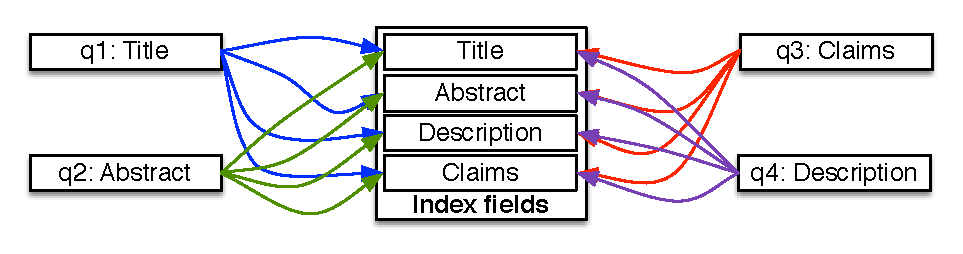
\includegraphics[width=8cm]{img/matching}
%\par\end{centering}
%\caption{Model of the index fields matching with queries .}
%\label{fig:IndexFields}
%\end{figure}





\section{Experimental Evaluation}
\label{sec:evaluation}
In this section, we discuss the results of the evaluation performed
on the query reformulation methods described above.

Figure \ref{fig:QE-qClaims-sAbstract-CLEF-2010} shows the results
obtained in terms of MAP and PRES for CLEF-IP 2010 for different numbers
of expanded terms $k$ on the x-axis (with $k=0$ using no QE, just
the baseline retrieval model). For lack of space we show only the
results of queries extracted from the claims and the abstract used
as source of query expansion. From these results, we make the following
observations: (i) for the two retrieval models (VSM and BM25), MMRQE
provides the best performance for both MAP and PRES (except for MAP,
where Rocchio BM25 provides better performance than MMRQE BM25), (ii)
for both MMRQE and Rocchio, the best performance is obtained while
adding no more than 50 terms to the original queries (adding more
terms may have no effect, or decrease the performance), and (iii)
exploiting external sources for query expansion provides poor performance
(IPC code definition and SynSets).

\begin{center}
\begin{figure}[h]
\begin{centering}
\includegraphics[width=4.3cm]{Results-CIKM2014/qClaims-sAbstract_MAP_2010}\includegraphics[width=4.3cm]{Results-CIKM2014/qClaims-sAbstract_PRES_2010}
\par\end{centering}
\caption{Results obtained while using the claims for querying and the abstract
as source of query expansion on the CLEF-IP 2010 dataset.}
\label{fig:QE-qClaims-sAbstract-CLEF-2010}
\end{figure}

\par\end{center}

To summarize all the results obtained over all the above configurations,
Figures~\ref{fig:MAP-CLEF2010},~\ref{fig:PRES-CLEF2010},~\ref{fig:MAP-CLEF2011},
and~\ref{fig:PRES-CLEF2011} show the performance obtained for all
the QE methods, while selecting the optimal number of terms used for
the expansion (number of terms that maximizes the performance for
each method). From these results, we first observe that the best section
to use for querying is the description section (see Figures \ref{fig:qDescription-MAP-CLEF-IP2010},
\ref{fig:qDescription-PRES-CLEF-IP2010}, \ref{fig:qDescription-MAP-CLEF-IP2011},
and \ref{fig:qDescription-PRES-CLEF-IP2011}). We attribute this to
the fact that the description section has more content along with
relevant terms that define the invention since a detailed summary
of the invention is described therein.

According to our experiments, the \textbf{best source for query expansion
is the claims section}. We attribute this to the fact that, the claims
contained not only relevant, but also, specific terminology, since
the scope of the invention is described therein. However, when querying
using the claims, other sources of query expansion provided better
performance. This may be because claims contained a lot of repetition 
and consequently, lack of the diversity necessary to capture similar inventions
that are described using synonyms or more specific or abstract terms.
It is interesting to notice that the description is not either a good
source for expansion, since its content is too broad, therefore, it
contains many irrelevant terms that hurt the performance.

As expected, we observed that query expansion is not useful for very
long queries (i.e. description), indicating that in advanced stages
of the patent application process, QE is not relevant. 
We also notice that using external sources for expansion such as the IPC code definitions,  
synsets from Wordnet gave poor performance.



\subsubsection{Discussion}

As recommended in \cite{Ganguly2011}
and confirmed in our own experimentation (not shown due to lack of
space), best QR performance results are also obtained when using few
documents in the PRF set (in our case, the top five gave the best
results).

\begin{comment}
Figure \ref{fig:DivImpactMMRQR} shows the impact of the diversity
parameter $\lambda$ on the performance of MMRQR. The results are
shown using BM25 retrieval model, and using abstract and claims for
querying. Throughout our experiments, we concluded that the best value
of $\lambda$ is 0.8, which indicates that few diversification in
term selection can provide some improvement. It is clear that if we
consider only diversification to select terms ($\lambda=0$), the
overall performance are significantly degraded. This is certainly
due to the fact that if we consider only diversified terms in the
query, there is a loss in the meaning of the query, and thus, we increase
the probability of retrieving irrelevant patents.

\begin{figure}[h]
\begin{centering}
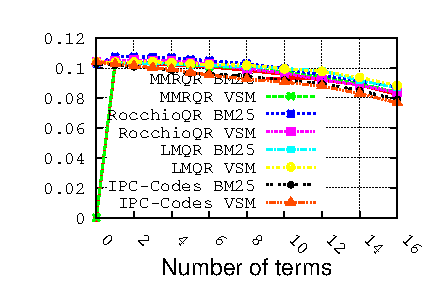
\includegraphics[width=3cm]{mmrqrResults-lambda/qAbstract-sDescription_MAP_2010}\includegraphics[width=3cm]{mmrqrResults-lambda/qAbstract-sDescription_PRES_2010}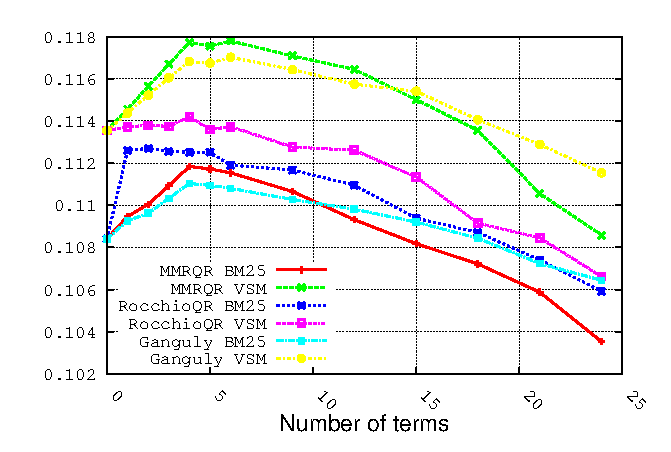
\includegraphics[width=3cm]{mmrqrResults-lambda/qClaims-sDescription_MAP_2010}\includegraphics[width=3cm]{mmrqrResults-lambda/qClaims-sDescription_PRES_2010}
\par\end{centering}

\caption{Impact of the diversity parameter $\lambda$ on the performance of
MMRQR on the CLEF-IP 2010 dataset.}
\label{fig:DivImpactMMRQR}
\end{figure}
\end{comment}



Figure \ref{fig:QR-qDescription-CLEF-2010} shows the results obtained
in terms of MAP and PRES for CLEF-IP 2010 for different numbers of
removed terms $k$ on the x-axis (with $k=0$ using no QR, just the
baseline retrieval model). For lack of space we show only the results
of queries extracted from the description. These results tell us mainly
two things: (i) for the two retrieval models, MMRQR provides the best
performance for both MAP and PRES, and (ii) for almost all methods,
the best performance is obtained when removing about 30 terms from
the original queries (in the case where the description is used for
querying). Removing more terms will decrease significantly the performance.

To summarize all the results obtained over all the above configurations,
Figures~\ref{fig:QR-PRES-CLEF-IP2010}, ~\ref{fig:QR-MAP-CLEF-IP2010},~\ref{fig:QR-PRES-CLEF-IP2011},
and~\ref{fig:QR-MAP-CLEF-IP2011} show the performance obtained for
all the QR methods, when selecting the optimal number of terms removed
from the original queries (number of terms removed that maximizes
the performance for each method).

From these results, we make the following observations: (i) query
reduction is very often not useful for short queries (i.e. title),
since no QR method outperforms significantly the baseline (i.e. No
QR), (ii) when dealing with very long query (i.e. description), BM25
based QR methods perform better than VSM based QR methods
%, and (iii) in general, MMRQR provides better performance than the other methods.






\begin{center}
\begin{figure}[t]
\begin{centering}
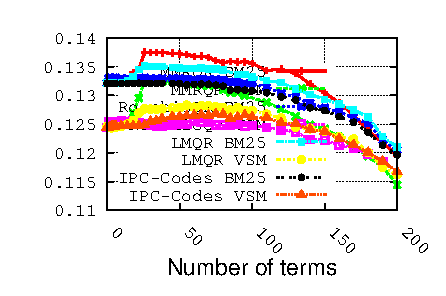
\includegraphics[width=4.3cm]{mmrqrResults/qDescription-sDescription_MAP_2010}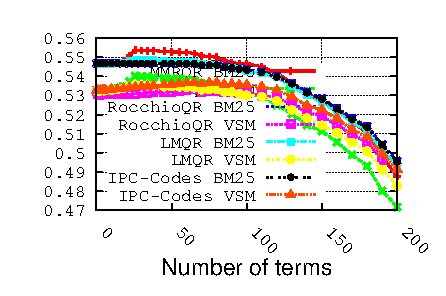
\includegraphics[width=4.3cm]{mmrqrResults/qDescription-sDescription_PRES_2010}
\par\end{centering}

\caption{Results obtained for QR while using the description for querying on
the CLEF-IP 2010 dataset.}


\label{fig:QR-qDescription-CLEF-2010}
\end{figure}

\par\end{center}


\section{Conclusion}

\label{sec:conclusion}

In this paper we analyzed general and specific QE and QR methods for
patent prior art search for partial (incomplete) patent applications
on two patent retrieval corpora, namely CLEF-IP 2010 and CLEF-IP 2011.
We demonstrated that QE methods are critical for short queries, i.e.
title, abstract, and claims, but useless for very long queries, i.e.
the description section. We also showed that claims is the best section
that works with QE both to query with and to use as a source of query
expansion terms, suggesting that claims should be written at early
stages of the patent application drafting so that they can be use
to performed patent prior art search. We also demonstrate that the
novel MMRQE method improves QE results in many cases. Future work
can look at more patent-specific methods of QE for prior art search
with partial patent applications and how they can be integrated with
methods like MMRQE.

Regarding QR methods, we showed that these techniques are effective
to some extent for claims and description sections, which are considered
the longest sections in a patent application. We also demonstrated
that our new QR method MMRQR improve both recall and precision in
many cases. Future work may consist of exploiting query quality predictors
to identify useless terms in a query using machine learning methods.

%We demonstrated that it reasonable to do prior art search 
%with partial applications, especially when combined with query expansion methods. 
%We also found that the patent specific fields are more suited as a source for expansion than other sources.
%We plan to further refine our approach by using
%a term weighting scheme for MMRQE. Other future work direction is to used MMR
%during query reduction to remove terms, which are not diversified
%in the query.




{ \scriptsize

\bibliographystyle{abbrv}
\bibliography{biblio}


}

\clearpage{}

\begin{figure*}[t]
\begin{centering}
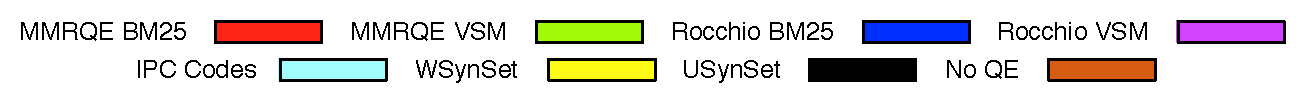
\includegraphics[width=17cm]{img/legendQE}
\par\end{centering}

\begin{centering}
\subfloat[Query Title.]{\begin{centering}
\includegraphics[width=8.6cm]{Results-CIKM2014/qTitle-MAP-CLEF-IP2010}
\par\end{centering}

}\subfloat[Query Abstract.]{\begin{centering}
\includegraphics[width=8.6cm]{Results-CIKM2014/qAbstract-MAP-CLEF-IP2010}
\par\end{centering}

}\subfloat[Query Claims.]{\begin{centering}
\includegraphics[width=8.6cm]{Results-CIKM2014/qClaims-MAP-CLEF-IP2010}
\par\end{centering}

}\subfloat[Query Description.]{\begin{centering}
\includegraphics[width=8.6cm]{Results-CIKM2014/qDescription-MAP-CLEF-IP2010}
\par\end{centering}

}\label{fig:qDescription-MAP-CLEF-IP2010}
\par\end{centering}

\caption{Mean Average Precision (MAP) for QE methods on CLEF-IP 2010 (for MMRQE
$\lambda=0.5$).}


\label{fig:MAP-CLEF2010}
\end{figure*}


\begin{figure*}[t]
\begin{centering}
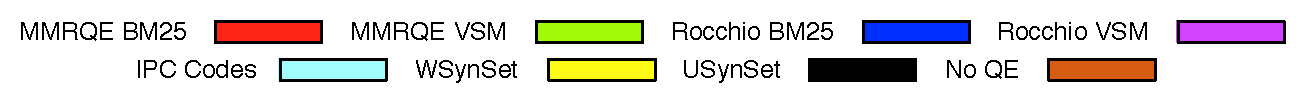
\includegraphics[width=17cm]{img/legendQE}
\par\end{centering}

\begin{centering}
\subfloat[Query Title.]{\begin{centering}
\includegraphics[width=8.6cm]{Results-CIKM2014/qTitle-PRES-CLEF-IP2010}
\par\end{centering}

}\subfloat[Query Abstract.]{\begin{centering}
\includegraphics[width=8.6cm]{Results-CIKM2014/qAbstract-PRES-CLEF-IP2010}
\par\end{centering}

}\subfloat[Query Claims.]{\begin{centering}
\includegraphics[width=8.6cm]{Results-CIKM2014/qClaims-PRES-CLEF-IP2010}
\par\end{centering}

}\subfloat[Query Description.]{\begin{centering}
\includegraphics[width=8.6cm]{Results-CIKM2014/qDescription-PRES-CLEF-IP2010}
\par\end{centering}

}\label{fig:qDescription-PRES-CLEF-IP2010}
\par\end{centering}

\caption{Patent Retrieval Evaluation Score (PRES) for QE methods on CLEF-IP
2010 (for MMRQE $\lambda=0.5$).}


\label{fig:PRES-CLEF2010}
\end{figure*}


\begin{figure*}[t]
\begin{centering}
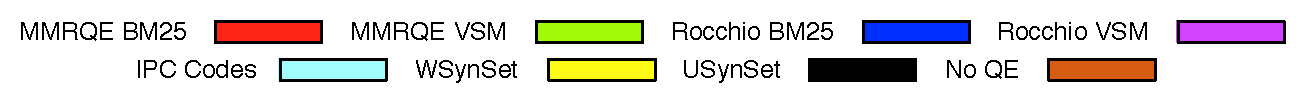
\includegraphics[width=17cm]{img/legendQE}
\par\end{centering}

\begin{centering}
\subfloat[Query Title.]{\begin{centering}
\includegraphics[width=8.6cm]{Results-CIKM2014/qTitle-MAP-CLEF-IP2011}
\par\end{centering}

}\subfloat[Query Abstract.]{\begin{centering}
\includegraphics[width=8.6cm]{Results-CIKM2014/qAbstract-MAP-CLEF-IP2011}
\par\end{centering}

}\subfloat[Query Claims.]{\begin{centering}
\includegraphics[width=8.6cm]{Results-CIKM2014/qClaims-MAP-CLEF-IP2011}
\par\end{centering}

}\subfloat[uery Description.]{\begin{centering}
\includegraphics[width=8.6cm]{Results-CIKM2014/qDescription-MAP-CLEF-IP2011}
\par\end{centering}

}\label{fig:qDescription-MAP-CLEF-IP2011}
\par\end{centering}

\caption{Mean Average Precision (MAP) for QE methods on CLEF-IP 2011 (for MMRQE
$\lambda=0.5$).}


\label{fig:MAP-CLEF2011}
\end{figure*}


\clearpage{}

\begin{figure*}[t]
\begin{centering}
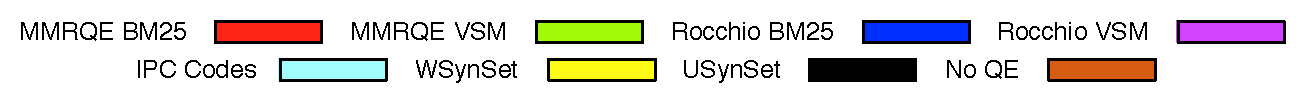
\includegraphics[width=17cm]{img/legendQE}
\par\end{centering}

\begin{centering}
\subfloat[Query Title.]{\begin{centering}
\includegraphics[width=8.4cm]{Results-CIKM2014/qTitle-PRES-CLEF-IP2011}
\par\end{centering}

}\subfloat[Query Abstract.]{\begin{centering}
\includegraphics[width=8.4cm]{Results-CIKM2014/qAbstract-PRES-CLEF-IP2011}
\par\end{centering}

}
\par\end{centering}

\begin{centering}
\subfloat[Query Claims.]{\begin{centering}
\includegraphics[width=8.4cm]{Results-CIKM2014/qClaims-PRES-CLEF-IP2011}
\par\end{centering}

}\subfloat[Query Description.]{\begin{centering}
\includegraphics[width=8.6cm]{Results-CIKM2014/qDescription-PRES-CLEF-IP2011}
\par\end{centering}

}\label{fig:qDescription-PRES-CLEF-IP2011}
\par\end{centering}

\caption{Patent Retrieval Evaluation Score (PRES) for QE methods on CLEF 2011
(for MMRQE $\lambda=0.5$).}


\label{fig:PRES-CLEF2011}
\end{figure*}


\begin{figure*}[t]
\begin{centering}
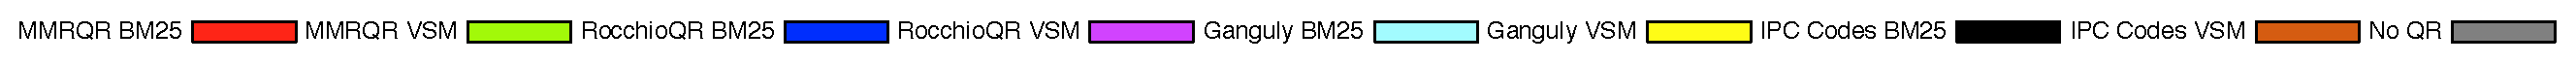
\includegraphics[width=15.5cm]{img/legendQR}
\par\end{centering}

\begin{centering}
\subfloat[Query Title.]{\begin{centering}
\includegraphics[width=4cm]{mmrqrResults/qTitle-MAP-CLEF-IP2010}
\par\end{centering}

}\subfloat[Query Abstract.]{\begin{centering}
\includegraphics[width=4cm]{mmrqrResults/qAbstract-MAP-CLEF-IP2010}
\par\end{centering}

}\subfloat[Query Claims.]{\begin{centering}
\includegraphics[width=4cm]{mmrqrResults/qClaims-MAP-CLEF-IP2010}
\par\end{centering}

}\subfloat[Query Description.]{\begin{centering}
\includegraphics[width=4cm]{mmrqrResults/qDescription-MAP-CLEF-IP2010}
\par\end{centering}

}
\par\end{centering}

\caption{Mean Average Precision (MAP) for QR methods on CLEF-IP 2010 (for MMRQR
$\lambda=0.8$).}


\label{fig:QR-PRES-CLEF-IP2010}
\end{figure*}


\begin{figure*}[t]
\begin{centering}
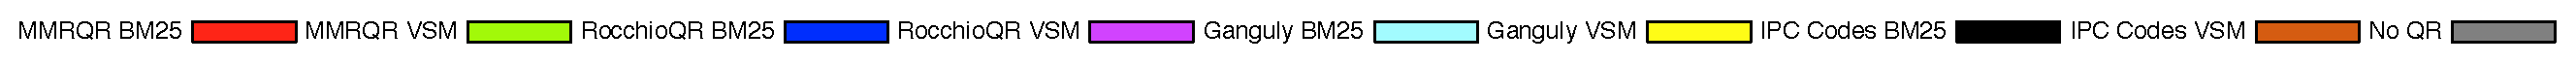
\includegraphics[width=15.5cm]{img/legendQR}
\par\end{centering}

\begin{centering}
\subfloat[Query Title.]{\begin{centering}
\includegraphics[width=4cm]{mmrqrResults/qTitle-PRES-CLEF-IP2010}
\par\end{centering}

}\subfloat[Query Abstract.]{\begin{centering}
\includegraphics[width=4cm]{mmrqrResults/qAbstract-PRES-CLEF-IP2010}
\par\end{centering}

}\subfloat[Query Claims.]{\begin{centering}
\includegraphics[width=4cm]{mmrqrResults/qClaims-PRES-CLEF-IP2010}
\par\end{centering}

}\subfloat[Query Description.]{\begin{centering}
\includegraphics[width=4cm]{mmrqrResults/qDescription-PRES-CLEF-IP2010}
\par\end{centering}

}
\par\end{centering}

\caption{Patent Retrieval Evaluation Score (PRES) for QR methods on CLEF 2010
(for MMRQR $\lambda=0.8$).}


\label{fig:QR-MAP-CLEF-IP2010}
\end{figure*}


\begin{figure*}[t]
\begin{centering}
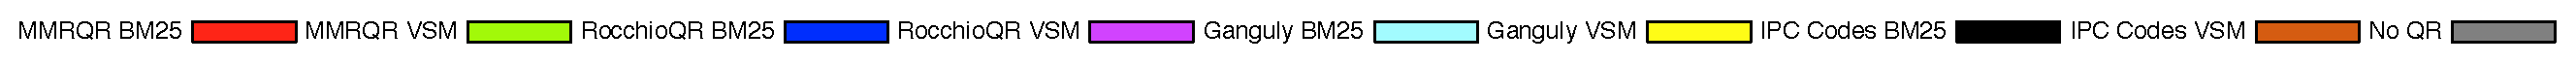
\includegraphics[width=15.5cm]{img/legendQR}
\par\end{centering}

\begin{centering}
\subfloat[Query Title.]{\begin{centering}
\includegraphics[width=4cm]{mmrqrResults/qTitle-MAP-CLEF-IP2011}
\par\end{centering}

}\subfloat[Query Abstract.]{\begin{centering}
\includegraphics[width=4cm]{mmrqrResults/qAbstract-MAP-CLEF-IP2011}
\par\end{centering}

}\subfloat[Query Claims.]{\begin{centering}
\includegraphics[width=4cm]{mmrqrResults/qClaims-MAP-CLEF-IP2011}
\par\end{centering}

}\subfloat[Query Description.]{\begin{centering}
\includegraphics[width=4cm]{mmrqrResults/qDescription-MAP-CLEF-IP2011}
\par\end{centering}

}
\par\end{centering}

\caption{Mean Average Precision (MAP) for QR methods on CLEF-IP 2011 (for MMRQR
$\lambda=0.8$).}


\label{fig:QR-PRES-CLEF-IP2011}
\end{figure*}


\begin{figure*}[t]
\begin{centering}
\includegraphics[width=15.5cm]{img/legendQR}
\par\end{centering}

\begin{centering}
\subfloat[Query Title.]{\begin{centering}
\includegraphics[width=4cm]{mmrqrResults/qTitle-PRES-CLEF-IP2011}
\par\end{centering}

}\subfloat[Query Abstract.]{\begin{centering}
\includegraphics[width=4cm]{mmrqrResults/qAbstract-PRES-CLEF-IP2011}
\par\end{centering}

}\subfloat[Query Claims.]{\begin{centering}
\includegraphics[width=4cm]{mmrqrResults/qClaims-PRES-CLEF-IP2011}
\par\end{centering}

}\subfloat[Query Description.]{\begin{centering}
\includegraphics[width=4cm]{mmrqrResults/qDescription-PRES-CLEF-IP2011}
\par\end{centering}

}
\par\end{centering}

\caption{Patent Retrieval Evaluation Score (PRES) for QR methods on CLEF 2011
(for MMRQR $\lambda=0.8$).}


\label{fig:QR-MAP-CLEF-IP2011}
\end{figure*}


\clearpage{}

\begin{comment}
\begin{figure*}[t]
\begin{centering}
\subfigure[{\tiny Query Title \& source Title.}]{\includegraphics[width=4.3cm]{Results-CIKM2014/qTitle-sTitle_MAP_2010.eps}}\subfigure[{\tiny Query Title \& source Abstract.}]{\includegraphics[width=4.3cm]{Results-CIKM2014/qTitle-sAbstract_MAP_2010.eps}}\subfigure[{\tiny Query Title \& source Claims.}]{\includegraphics[width=4.3cm]{Results-CIKM2014/qTitle-sClaims_MAP_2010.eps}}\subfigure[{\tiny Query Title \& source Descrip.}]{\includegraphics[width=4.3cm]{Results-CIKM2014/qTitle-sDescription_MAP_2010.eps}} 
\par\end{centering}

\begin{centering}
\subfigure[{\tiny Query Abstract \& source Title.}]{\includegraphics[width=4.3cm]{Results-CIKM2014/qAbstract-sTitle_MAP_2010.eps}}\subfigure[{\tiny Query Abstract \& source Abstract.}]{\includegraphics[width=4.3cm]{Results-CIKM2014/qAbstract-sAbstract_MAP_2010.eps}}\subfigure[{\tiny Query Abstract \& source Claims.}]{\includegraphics[width=4.3cm]{Results-CIKM2014/qAbstract-sClaims_MAP_2010.eps}}\subfigure[{\tiny Query Abstract \& source Descrip.}]{\includegraphics[width=4.3cm]{Results-CIKM2014/qAbstract-sDescription_MAP_2010.eps}} 
\par\end{centering}

\begin{centering}
\subfigure[{\tiny Query Claims \& source Title.}]{\includegraphics[width=4.3cm]{Results-CIKM2014/qClaims-sTitle_MAP_2010.eps}}\subfigure[{\tiny Query Claims \& source Abstract.}]{\includegraphics[width=4.3cm]{Results-CIKM2014/qClaims-sAbstract_MAP_2010.eps}}\subfigure[{\tiny Query Claims \& source Claims.}]{\includegraphics[width=4.3cm]{Results-CIKM2014/qClaims-sClaims_MAP_2010.eps}}\subfigure[{\tiny Query Claims \& source Descrip.}]{\includegraphics[width=4.3cm]{Results-CIKM2014/qClaims-sDescription_MAP_2010.eps}}
\subfigure[{\tiny Query Descrip \& source Title.}]{\includegraphics[width=4.3cm]{Results-CIKM2014/qDescription-sTitle_MAP_2010.eps}}\subfigure[{\tiny Query Descrip \& source Abstract.}]{\includegraphics[width=4.3cm]{Results-CIKM2014/qDescription-sAbstract_MAP_2010.eps}}\subfigure[{\tiny Query Descrip \& source Claims.}]{\includegraphics[width=4.3cm]{Results-CIKM2014/qDescription-sClaims_MAP_2010.eps}}\subfigure[{\tiny Query Descrip \& source Descrip.}]{\includegraphics[width=4.3cm]{Results-CIKM2014/qDescription-sDescription_MAP_2010.eps}} 
\par\end{centering}

\caption{Mean Average Precision (MAP) on CLEF-2010 (for MMRQE $\lambda=0.5$).}


\label{fig:MAP-CLEF2010-1}
\end{figure*}


\begin{figure*}
\begin{centering}
\subfigure[{\tiny Query Title \& source Title.}]{\includegraphics[width=4.3cm]{Results-CIKM2014/qTitle-sTitle_PRES_2010.eps}}\subfigure[{\tiny Query Title \& source Abstract.}]{\includegraphics[width=4.3cm]{Results-CIKM2014/qTitle-sAbstract_PRES_2010.eps}}\subfigure[{\tiny Query Title \& source Claims.}]{\includegraphics[width=4.3cm]{Results-CIKM2014/qTitle-sClaims_PRES_2010.eps}}\subfigure[{\tiny Query Title \& source Descrip.}]{\includegraphics[width=4.3cm]{Results-CIKM2014/qTitle-sDescription_PRES_2010.eps}} 
\par\end{centering}

\begin{centering}
\subfigure[{\tiny Query Abstract \& source Title.}]{\includegraphics[width=4.3cm]{Results-CIKM2014/qAbstract-sTitle_PRES_2010.eps}}\subfigure[{\tiny Query Abstract \& source Abstract.}]{\includegraphics[width=4.3cm]{Results-CIKM2014/qAbstract-sAbstract_PRES_2010.eps}}\subfigure[{\tiny Query Abstract \& source Claims.}]{\includegraphics[width=4.3cm]{Results-CIKM2014/qAbstract-sClaims_PRES_2010.eps}}\subfigure[{\tiny Query Abstract \& source Descrip.}]{\includegraphics[width=4.3cm]{Results-CIKM2014/qAbstract-sDescription_PRES_2010.eps}} 
\par\end{centering}

\begin{centering}
\subfigure[{\tiny Query Claims \& source Title.}]{\includegraphics[width=4.3cm]{Results-CIKM2014/qClaims-sTitle_PRES_2010.eps}}\subfigure[{\tiny Query Claims \& source Abstract.}]{\includegraphics[width=4.3cm]{Results-CIKM2014/qClaims-sAbstract_PRES_2010.eps}}\subfigure[{\tiny Query Claims \& source Claims.}]{\includegraphics[width=4.3cm]{Results-CIKM2014/qClaims-sClaims_PRES_2010.eps}}\subfigure[{\tiny Query Claims \& source Descrip.}]{\includegraphics[width=4.3cm]{Results-CIKM2014/qClaims-sDescription_PRES_2010.eps}}
\subfigure[{\tiny Query Descrip \& source Title.}]{\includegraphics[width=4.3cm]{Results-CIKM2014/qDescription-sTitle_PRES_2010.eps}}\subfigure[{\tiny Query Descrip \& source Abstract.}]{\includegraphics[width=4.3cm]{Results-CIKM2014/qDescription-sAbstract_PRES_2010.eps}}\subfigure[{\tiny Query Descrip \& source Claims.}]{\includegraphics[width=4.3cm]{Results-CIKM2014/qDescription-sClaims_PRES_2010.eps}}\subfigure[{\tiny Query Descrip \& source Descrip.}]{\includegraphics[width=4.3cm]{Results-CIKM2014/qDescription-sDescription_PRES_2010.eps}} 
\par\end{centering}

\caption{Patent Retrieval Evaluation Score (PRES) on CLEF-2010 (for MMRQE $\lambda=0.5$).}


\label{fig:PRES-CLEF2010-1} 
\end{figure*}


\begin{figure*}[t]
\begin{centering}
\subfigure[{\tiny Query Title \& source Title.}]{\includegraphics[width=4.3cm]{Results-CIKM2014/qTitle-sTitle_MAP_2011.eps}}\subfigure[{\tiny Query Title \& source Abstract.}]{\includegraphics[width=4.3cm]{Results-CIKM2014/qTitle-sAbstract_MAP_2011.eps}}\subfigure[{\tiny Query Title \& source Claims.}]{\includegraphics[width=4.3cm]{Results-CIKM2014/qTitle-sClaims_MAP_2011.eps}}\subfigure[{\tiny Query Title \& source Descrip.}]{\includegraphics[width=4.3cm]{Results-CIKM2014/qTitle-sDescription_MAP_2011.eps}} 
\par\end{centering}

\begin{centering}
\subfigure[{\tiny Query Abstract \& source Title.}]{\includegraphics[width=4.3cm]{Results-CIKM2014/qAbstract-sTitle_MAP_2011.eps}}\subfigure[{\tiny Query Abstract \& source Abstract.}]{\includegraphics[width=4.3cm]{Results-CIKM2014/qAbstract-sAbstract_MAP_2011.eps}}\subfigure[{\tiny Query Abstract \& source Claims.}]{\includegraphics[width=4.3cm]{Results-CIKM2014/qAbstract-sClaims_MAP_2011.eps}}\subfigure[{\tiny Query Abstract \& source Descrip.}]{\includegraphics[width=4.3cm]{Results-CIKM2014/qAbstract-sDescription_MAP_2011.eps}} 
\par\end{centering}

\begin{centering}
\subfigure[{\tiny Query Claims \& source Title.}]{\includegraphics[width=4.3cm]{Results-CIKM2014/qClaims-sTitle_MAP_2011.eps}}\subfigure[{\tiny Query Claims \& source Abstract.}]{\includegraphics[width=4.3cm]{Results-CIKM2014/qClaims-sAbstract_MAP_2011.eps}}\subfigure[{\tiny Query Claims \& source Claims.}]{\includegraphics[width=4.3cm]{Results-CIKM2014/qClaims-sClaims_MAP_2011.eps}}\subfigure[{\tiny Query Claims \& source Descrip.}]{\includegraphics[width=4.3cm]{Results-CIKM2014/qClaims-sDescription_MAP_2011.eps}}
\subfigure[{\tiny Query Descrip \& source Title.}]{\includegraphics[width=4.3cm]{Results-CIKM2014/qDescription-sTitle_MAP_2011.eps}}\subfigure[{\tiny Query Descrip \& source Abstract.}]{\includegraphics[width=4.3cm]{Results-CIKM2014/qDescription-sAbstract_MAP_2011.eps}}\subfigure[{\tiny Query Descrip \& source Claims.}]{\includegraphics[width=4.3cm]{Results-CIKM2014/qDescription-sClaims_MAP_2011.eps}}\subfigure[{\tiny Query Descrip \& source Descrip.}]{\includegraphics[width=4.3cm]{Results-CIKM2014/qDescription-sDescription_MAP_2011.eps}} 
\par\end{centering}

\caption{Mean Average Precision (MAP) on CLEF-2011 (for MMRQE $\lambda=0.5$).}
\end{figure*}


\begin{figure*}
\begin{centering}
\subfigure[{\tiny Query Title \& source Title.}]{\includegraphics[width=4.3cm]{Results-CIKM2014/qTitle-sTitle_PRES_2011.eps}}\subfigure[{\tiny Query Title \& source Abstract.}]{\includegraphics[width=4.3cm]{Results-CIKM2014/qTitle-sAbstract_PRES_2011.eps}}\subfigure[{\tiny Query Title \& source Claims.}]{\includegraphics[width=4.3cm]{Results-CIKM2014/qTitle-sClaims_PRES_2011.eps}}\subfigure[{\tiny Query Title \& source Descrip.}]{\includegraphics[width=4.3cm]{Results-CIKM2014/qTitle-sDescription_PRES_2011.eps}} 
\par\end{centering}

\begin{centering}
\subfigure[{\tiny Query Abstract \& source Title.}]{\includegraphics[width=4.3cm]{Results-CIKM2014/qAbstract-sTitle_PRES_2011.eps}}\subfigure[{\tiny Query Abstract \& source Abstract.}]{\includegraphics[width=4.3cm]{Results-CIKM2014/qAbstract-sAbstract_PRES_2011.eps}}\subfigure[{\tiny Query Abstract \& source Claims.}]{\includegraphics[width=4.3cm]{Results-CIKM2014/qAbstract-sClaims_PRES_2011.eps}}\subfigure[{\tiny Query Abstract \& source Descrip.}]{\includegraphics[width=4.3cm]{Results-CIKM2014/qAbstract-sDescription_PRES_2011.eps}} 
\par\end{centering}

\begin{centering}
\subfigure[{\tiny Query Claims \& source Title.}]{\includegraphics[width=4.3cm]{Results-CIKM2014/qClaims-sTitle_PRES_2011.eps}}\subfigure[{\tiny Query Claims \& source Abstract.}]{\includegraphics[width=4.3cm]{Results-CIKM2014/qClaims-sAbstract_PRES_2011.eps}}\subfigure[{\tiny Query Claims \& source Claims.}]{\includegraphics[width=4.3cm]{Results-CIKM2014/qClaims-sClaims_PRES_2011.eps}}\subfigure[{\tiny Query Claims \& source Descrip.}]{\includegraphics[width=4.3cm]{Results-CIKM2014/qClaims-sDescription_PRES_2011.eps}}
\subfigure[{\tiny Query Descrip \& source Title.}]{\includegraphics[width=4.3cm]{Results-CIKM2014/qDescription-sTitle_PRES_2011.eps}}\subfigure[{\tiny Query Descrip \& source Abstract.}]{\includegraphics[width=4.3cm]{Results-CIKM2014/qDescription-sAbstract_PRES_2011.eps}}\subfigure[{\tiny Query Descrip \& source Claims.}]{\includegraphics[width=4.3cm]{Results-CIKM2014/qDescription-sClaims_PRES_2011.eps}}\subfigure[{\tiny Query Descrip \& source Descrip.}]{\includegraphics[width=4.3cm]{Results-CIKM2014/qDescription-sDescription_PRES_2011.eps}} 
\par\end{centering}

\caption{Patent Retrieval Evaluation Score (PRES) on CLEF-2011 (for MMRQE $\lambda=0.5$).}
\end{figure*}
\end{comment}


\clearpage{}

\begin{comment}
\begin{figure*}[t]
\begin{centering}
\subfigure[{Query Title.}]{\includegraphics[width=4.3cm]{mmrqrResults/qTitle-sDescription_MAP_2010.eps}}\subfigure[{Query Abstract.}]{\includegraphics[width=4.3cm]{mmrqrResults/qAbstract-sDescription_MAP_2010.eps}}\subfigure[{Query Claims.}]{\includegraphics[width=4.3cm]{mmrqrResults/qClaims-sDescription_MAP_2010.eps}}
\subfigure[{Query Description.}]{\includegraphics[width=4.3cm]{mmrqrResults/qDescription-sDescription_MAP_2010.eps}} 
\par\end{centering}

\caption{Mean Average Precision (MAP) for MMRQR on CLEF-2010 (for MMRQE $\lambda=0.8$).}
\end{figure*}


\begin{figure*}
\begin{centering}
\subfigure[{ Query Title.}]{\includegraphics[width=4.3cm]{mmrqrResults/qTitle-sDescription_PRES_2010.eps}}\subfigure[{Query Abstract.}]{\includegraphics[width=4.3cm]{mmrqrResults/qAbstract-sDescription_PRES_2010.eps}}\subfigure[{Query Claims.}]{\includegraphics[width=4.3cm]{mmrqrResults/qClaims-sDescription_PRES_2010.eps}}
\subfigure[{Query Description.}]{\includegraphics[width=4.3cm]{mmrqrResults/qDescription-sDescription_PRES_2010.eps}} 
\par\end{centering}

\caption{Patent Retrieval Evaluation Score (PRES) for MMRQR on CLEF-2010 (for
MMRQE $\lambda=0.8$).}
\end{figure*}


\begin{figure*}[t]
\begin{centering}
\subfigure[{Query Title.}]{\includegraphics[width=4.3cm]{mmrqrResults/qTitle-sDescription_MAP_2011.eps}}\subfigure[{Query Abstract.}]{\includegraphics[width=4.3cm]{mmrqrResults/qAbstract-sDescription_MAP_2011.eps}}\subfigure[{Query Claims.}]{\includegraphics[width=4.3cm]{mmrqrResults/qClaims-sDescription_MAP_2011.eps}}
\subfigure[{Query Description.}]{\includegraphics[width=4.3cm]{mmrqrResults/qDescription-sDescription_MAP_2011.eps}} 
\par\end{centering}

\caption{Mean Average Precision (MAP) for MMRQR on CLEF-2011 (for MMRQE $\lambda=0.8$).}
\end{figure*}


\begin{figure*}
\begin{centering}
\subfigure[{ Query Title.}]{\includegraphics[width=4.3cm]{mmrqrResults/qTitle-sDescription_PRES_2011.eps}}\subfigure[{Query Abstract.}]{\includegraphics[width=4.3cm]{mmrqrResults/qAbstract-sDescription_PRES_2011.eps}}\subfigure[{Query Claims.}]{\includegraphics[width=4.3cm]{mmrqrResults/qClaims-sDescription_PRES_2011.eps}}
\subfigure[{Query Description.}]{\includegraphics[width=4.3cm]{mmrqrResults/qDescription-sDescription_PRES_2011.eps}} 
\par\end{centering}

\caption{Patent Retrieval Evaluation Score (PRES) for MMRQR on CLEF-2011 (for
MMRQE $\lambda=0.8$).}
\end{figure*}
\end{comment}

\end{document}
